\chapter{The Burglary}

The day following that on which the conversation we have related took
place, the Count of Monte Cristo set out for Auteuil, accompanied by
Ali and several attendants, and also taking with him some horses whose
qualities he was desirous of ascertaining. He was induced to undertake
this journey, of which the day before he had not even thought and which
had not occurred to Andrea either, by the arrival of Bertuccio from
Normandy with intelligence respecting the house and sloop. The house
was ready, and the sloop which had arrived a week before lay at anchor
in a small creek with her crew of six men, who had observed all the
requisite formalities and were ready again to put to sea.

The count praised Bertuccio’s zeal, and ordered him to prepare for a
speedy departure, as his stay in France would not be prolonged more
than a month.

“Now,” said he, “I may require to go in one night from Paris to
Tréport; let eight fresh horses be in readiness on the road, which will
enable me to go fifty leagues in ten hours.”

“Your highness had already expressed that wish,” said Bertuccio, “and
the horses are ready. I have bought them, and stationed them myself at
the most desirable posts, that is, in villages, where no one generally
stops.”

“That’s well,” said Monte Cristo; “I remain here a day or two—arrange
accordingly.”

As Bertuccio was leaving the room to give the requisite orders,
Baptistin opened the door: he held a letter on a silver waiter.

“What are you doing here?” asked the count, seeing him covered with
dust; “I did not send for you, I think?”

Baptistin, without answering, approached the count, and presented the
letter. “Important and urgent,” said he.

The count opened the letter, and read:

\begin{quote}
{\small“‘M. de Monte Cristo is apprised that this night a man will enter his
house in the Champs-Élysées with the intention of carrying off some
papers supposed to be in the secretaire in the dressing-room. The
count’s well-known courage will render unnecessary the aid of the
police, whose interference might seriously affect him who sends this
advice. The count, by any opening from the bedroom, or by concealing
himself in the dressing-room, would be able to defend his property
himself. Many attendants or apparent precautions would prevent the
villain from the attempt, and M. de Monte Cristo would lose the
opportunity of discovering an enemy whom chance has revealed to him who
now sends this warning to the count,—a warning he might not be able to
send another time, if this first attempt should fail and another be
made.’”}
\end{quote}

The count’s first idea was that this was an artifice—a gross deception,
to draw his attention from a minor danger in order to expose him to a
greater. He was on the point of sending the letter to the commissary of
police, notwithstanding the advice of his anonymous friend, or perhaps
because of that advice, when suddenly the idea occurred to him that it
might be some personal enemy, whom he alone should recognize and over
whom, if such were the case, he alone would gain any advantage, as
Fiesco\footnote[17]{The Genoese conspirator.} had done over the Moor
who would have killed him. We know the count’s vigorous and daring
mind, denying anything to be impossible, with that energy which marks
the great man.

From his past life, from his resolution to shrink from nothing, the
count had acquired an inconceivable relish for the contests in which he
had engaged, sometimes against nature, that is to say, against God, and
sometimes against the world, that is, against the devil.

“They do not want my papers,” said Monte Cristo, “they want to kill me;
they are no robbers, but assassins. I will not allow the prefect of
police to interfere with my private affairs. I am rich enough,
forsooth, to distribute his authority on this occasion.”

The count recalled Baptistin, who had left the room after delivering
the letter.

“Return to Paris,” said he; “assemble the servants who remain there. I
want all my household at Auteuil.”

“But will no one remain in the house, my lord?” asked Baptistin.

“Yes, the porter.”

“My lord will remember that the lodge is at a distance from the house.”

“Well?”

“The house might be stripped without his hearing the least noise.”

“By whom?”

“By thieves.”

“You are a fool, M. Baptistin. Thieves might strip the house—it would
annoy me less than to be disobeyed.” Baptistin bowed.

\begin{figure}[ht]
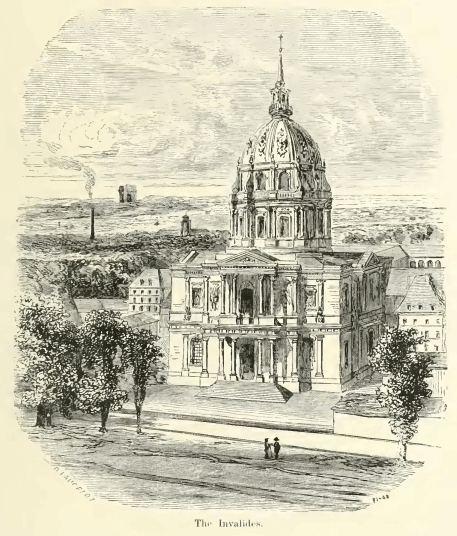
\includegraphics[width=\textwidth]{40150m.jpg}
\end{figure}

“You understand me?” said the count. “Bring your comrades here, one and
all; but let everything remain as usual, only close the shutters of the
ground floor.”

“And those of the first floor?”

“You know they are never closed. Go!”

The count signified his intention of dining alone, and that no one but
Ali should attend him. Having dined with his usual tranquillity and
moderation, the count, making a signal to Ali to follow him, went out
by the side-gate and on reaching the Bois de Boulogne turned,
apparently without design towards Paris and at twilight; found himself
opposite his house in the Champs-Élysées. All was dark; one solitary,
feeble light was burning in the porter’s lodge, about forty paces
distant from the house, as Baptistin had said.

Monte Cristo leaned against a tree, and with that scrutinizing glance
which was so rarely deceived, looked up and down the avenue, examined
the passers-by, and carefully looked down the neighboring streets, to
see that no one was concealed. Ten minutes passed thus, and he was
convinced that no one was watching him. He hastened to the side-door
with Ali, entered hurriedly, and by the servants’ staircase, of which
he had the key, gained his bedroom without opening or disarranging a
single curtain, without even the porter having the slightest suspicion
that the house, which he supposed empty, contained its chief occupant.

Arrived in his bedroom, the count motioned to Ali to stop; then he
passed into the dressing-room, which he examined. Everything appeared
as usual—the precious secretaire in its place, and the key in the
secretaire. He double locked it, took the key, returned to the bedroom
door, removed the double staple of the bolt, and went in. Meanwhile Ali
had procured the arms the count required—namely, a short carbine and a
pair of double-barrelled pistols, with which as sure an aim might be
taken as with a single-barrelled one. Thus armed, the count held the
lives of five men in his hands. It was about half-past nine.

The count and Ali ate in haste a crust of bread and drank a glass of
Spanish wine; then Monte Cristo slipped aside one of the movable
panels, which enabled him to see into the adjoining room. He had within
his reach his pistols and carbine, and Ali, standing near him, held one
of the small Arabian hatchets, whose form has not varied since the
Crusades. Through one of the windows of the bedroom, on a line with
that in the dressing-room, the count could see into the street.

Two hours passed thus. It was intensely dark; still Ali, thanks to his
wild nature, and the count, thanks doubtless to his long confinement,
could distinguish in the darkness the slightest movement of the trees.
The little light in the lodge had long been extinct. It might be
expected that the attack, if indeed an attack was projected, would be
made from the staircase of the ground floor, and not from a window; in
Monte Cristo’s opinion, the villains sought his life, not his money. It
would be his bedroom they would attack, and they must reach it by the
back staircase, or by the window in the dressing-room.

The clock of the Invalides struck a quarter to twelve; the west wind
bore on its moistened gusts the doleful vibration of the three strokes.

\begin{figure}[ht]
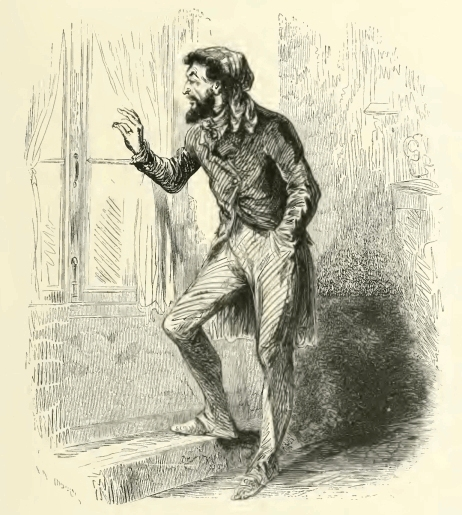
\includegraphics[width=\textwidth]{40152m.jpg}
\end{figure}

As the last stroke died away, the count thought he heard a slight noise
in the dressing-room; this first sound, or rather this first grinding,
was followed by a second, then a third; at the fourth, the count knew
what to expect. A firm and well-practised hand was engaged in cutting
the four sides of a pane of glass with a diamond. The count felt his
heart beat more rapidly.

Inured as men may be to danger, forewarned as they may be of peril,
they understand, by the fluttering of the heart and the shuddering of
the frame, the enormous difference between a dream and a reality,
between the project and the execution. However, Monte Cristo only made
a sign to apprise Ali, who, understanding that danger was approaching
from the other side, drew nearer to his master. Monte Cristo was eager
to ascertain the strength and number of his enemies.

The window whence the noise proceeded was opposite the opening by which
the count could see into the dressing-room. He fixed his eyes on that
window—he distinguished a shadow in the darkness; then one of the panes
became quite opaque, as if a sheet of paper were stuck on the outside,
then the square cracked without falling. Through the opening an arm was
passed to find the fastening, then a second; the window turned on its
hinges, and a man entered. He was alone.

“That’s a daring rascal,” whispered the count.

At that moment Ali touched him slightly on the shoulder. He turned; Ali
pointed to the window of the room in which they were, facing the
street.

“I see!” said he, “there are two of them; one does the work while the
other stands guard.” He made a sign to Ali not to lose sight of the man
in the street, and turned to the one in the dressing-room.

The glass-cutter had entered, and was feeling his way, his arms
stretched out before him. At last he appeared to have made himself
familiar with his surroundings. There were two doors; he bolted them
both.

When he drew near to the bedroom door, Monte Cristo expected that he
was coming in, and raised one of his pistols; but he simply heard the
sound of the bolts sliding in their copper rings. It was only a
precaution. The nocturnal visitor, ignorant of the fact that the count
had removed the staples, might now think himself at home, and pursue
his purpose with full security. Alone and free to act as he wished, the
man then drew from his pocket something which the count could not
discern, placed it on a stand, then went straight to the secretaire,
felt the lock, and contrary to his expectation found that the key was
missing. But the glass-cutter was a prudent man who had provided for
all emergencies. The count soon heard the rattling of a bunch of
skeleton keys, such as the locksmith brings when called to force a
lock, and which thieves call nightingales, doubtless from the music of
their nightly song when they grind against the bolt.

“Ah, ha,” whispered Monte Cristo with a smile of disappointment, “he is
only a thief.”

But the man in the dark could not find the right key. He reached the
instrument he had placed on the stand, touched a spring, and
immediately a pale light, just bright enough to render objects
distinct, was reflected on his hands and countenance.

“By heavens,” exclaimed Monte Cristo, starting back, “it is——”

Ali raised his hatchet.

“Don’t stir,” whispered Monte Cristo, “and put down your hatchet; we
shall require no arms.”

\begin{figure}[ht]
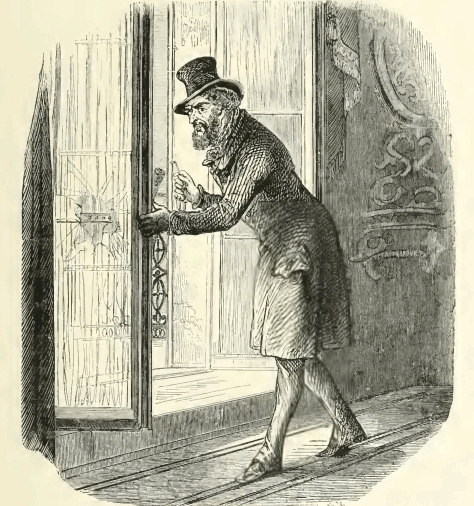
\includegraphics[width=\textwidth]{40154m.jpg}
\end{figure}

Then he added some words in a low tone, for the exclamation which
surprise had drawn from the count, faint as it had been, had startled
the man who remained in the pose of the old knife-grinder.

It was an order the count had just given, for immediately Ali went
noiselessly, and returned, bearing a black dress and a three-cornered
hat. Meanwhile Monte Cristo had rapidly taken off his greatcoat,
waistcoat, and shirt, and one might distinguish by the glimmering
through the open panel that he wore a pliant tunic of steel mail, of
which the last in France, where daggers are no longer dreaded, was worn
by King Louis XVI., who feared the dagger at his breast, and whose head
was cleft with a hatchet. The tunic soon disappeared under a long
cassock, as did his hair under a priest’s wig; the three-cornered hat
over this effectually transformed the count into an abbé.

The man, hearing nothing more, stood erect, and while Monte Cristo was
completing his disguise had advanced straight to the secretaire, whose
lock was beginning to crack under his nightingale.

“Try again,” whispered the count, who depended on the secret spring,
which was unknown to the picklock, clever as he might be—“try again,
you have a few minutes’ work there.”

And he advanced to the window. The man whom he had seen seated on a
fence had got down, and was still pacing the street; but, strange as it
appeared, he cared not for those who might pass from the avenue of the
Champs-Élysées or by the Faubourg Saint-Honoré; his attention was
engrossed with what was passing at the count’s, and his only aim
appeared to be to discern every movement in the dressing-room.

Monte Cristo suddenly struck his finger on his forehead and a smile
passed over his lips; then drawing near to Ali, he whispered:

“Remain here, concealed in the dark, and whatever noise you hear,
whatever passes, only come in or show yourself if I call you.”

Ali bowed in token of strict obedience. Monte Cristo then drew a
lighted taper from a closet, and when the thief was deeply engaged with
his lock, silently opened the door, taking care that the light should
shine directly on his face. The door opened so quietly that the thief
heard no sound; but, to his astonishment, the room was suddenly
illuminated. He turned.

“Ah, good-evening, my dear M. Caderousse,” said Monte Cristo; “what are
you doing here, at such an hour?”

\begin{figure}[ht]
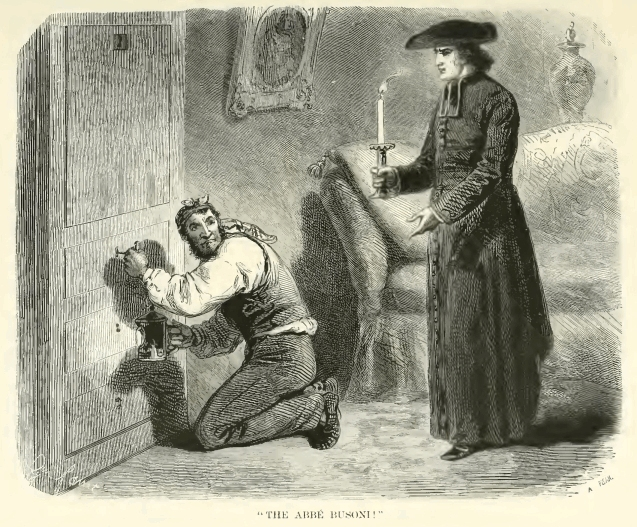
\includegraphics[width=\textwidth]{40156m.jpg}
\end{figure}

“The Abbé Busoni!” exclaimed Caderousse; and, not knowing how this
strange apparition could have entered when he had bolted the doors, he
let fall his bunch of keys, and remained motionless and stupefied. The
count placed himself between Caderousse and the window, thus cutting
off from the thief his only chance of retreat.

“The Abbé Busoni!” repeated Caderousse, fixing his haggard gaze on the
count.

“Yes, undoubtedly, the Abbé Busoni himself,” replied Monte Cristo. “And
I am very glad you recognize me, dear M. Caderousse; it proves you have
a good memory, for it must be about ten years since we last met.”

This calmness of Busoni, combined with his irony and boldness,
staggered Caderousse.

“The abbé, the abbé!” murmured he, clenching his fists, and his teeth
chattering.

“So you would rob the Count of Monte Cristo?” continued the false abbé.

“Reverend sir,” murmured Caderousse, seeking to regain the window,
which the count pitilessly blocked—“reverend sir, I don’t know—believe
me—I take my oath——”

“A pane of glass out,” continued the count, “a dark lantern, a bunch of
false keys, a secretaire half forced—it is tolerably evident——”

Caderousse was choking; he looked around for some corner to hide in,
some way of escape.

“Come, come,” continued the count, “I see you are still the same,—an
assassin.”

“Reverend sir, since you know everything, you know it was not I—it was
La Carconte; that was proved at the trial, since I was only condemned
to the galleys.”

“Is your time, then, expired, since I find you in a fair way to return
there?”

“No, reverend sir; I have been liberated by someone.”

“That someone has done society a great kindness.”

“Ah,” said Caderousse, “I had promised——”

“And you are breaking your promise!” interrupted Monte Cristo.

“Alas, yes!” said Caderousse very uneasily.

“A bad relapse, that will lead you, if I mistake not, to the Place de
Grève. So much the worse, so much the worse—\textit{diavolo!} as they say in
my country.”

“Reverend sir, I am impelled——”

“Every criminal says the same thing.”

“Poverty——”

“Pshaw!” said Busoni disdainfully; “poverty may make a man beg, steal a
loaf of bread at a baker’s door, but not cause him to open a secretaire
in a house supposed to be inhabited. And when the jeweller Johannes had
just paid you 45,000 francs for the diamond I had given you, and you
killed him to get the diamond and the money both, was that also
poverty?”

“Pardon, reverend sir,” said Caderousse; “you have saved my life once,
save me again!”

“That is but poor encouragement.”

“Are you alone, reverend sir, or have you there soldiers ready to seize
me?”

“I am alone,” said the abbé, “and I will again have pity on you, and
will let you escape, at the risk of the fresh miseries my weakness may
lead to, if you tell me the truth.”

“Ah, reverend sir,” cried Caderousse, clasping his hands, and drawing
nearer to Monte Cristo, “I may indeed say you are my deliverer!”

“You mean to say you have been freed from confinement?”

“Yes, that is true, reverend sir.”

“Who was your liberator?”

“An Englishman.”

“What was his name?”

“Lord Wilmore.”

“I know him; I shall know if you lie.”

“Ah, reverend sir, I tell you the simple truth.”

“Was this Englishman protecting you?”

“No, not me, but a young Corsican, my companion.”

“What was this young Corsican’s name?”

“Benedetto.”

“Is that his Christian name?”

“He had no other; he was a foundling.”

“Then this young man escaped with you?”

“He did.”

“In what way?”

“We were working at Saint-Mandrier, near Toulon. Do you know
Saint-Mandrier?”

“I do.”

“In the hour of rest, between noon and one o’clock——”

“Galley-slaves having a nap after dinner! We may well pity the poor
fellows!” said the abbé.

“Nay,” said Caderousse, “one can’t always work—one is not a dog.”

“So much the better for the dogs,” said Monte Cristo.

“While the rest slept, then, we went away a short distance; we severed
our fetters with a file the Englishman had given us, and swam away.”

“And what is become of this Benedetto?”

“I don’t know.”

“You ought to know.”

“No, in truth; we parted at Hyères.” And, to give more weight to his
protestation, Caderousse advanced another step towards the abbé, who
remained motionless in his place, as calm as ever, and pursuing his
interrogation.

“You lie,” said the Abbé Busoni, with a tone of irresistible authority.

“Reverend sir!”

“You lie! This man is still your friend, and you, perhaps, make use of
him as your accomplice.”

\begin{figure}[ht]
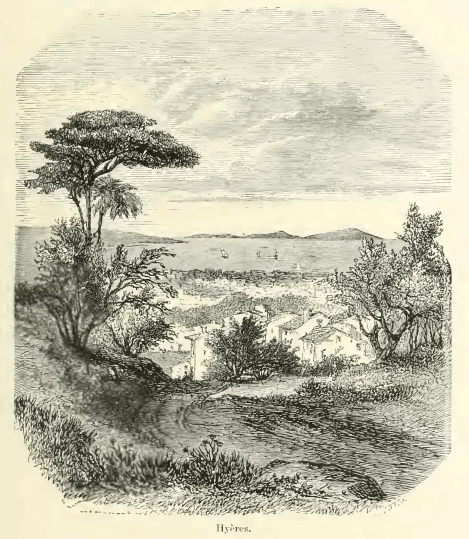
\includegraphics[width=\textwidth]{40160m.jpg}
\end{figure}

“Oh, reverend sir!”

“Since you left Toulon what have you lived on? Answer me!”

“On what I could get.”

“You lie,” repeated the abbé a third time, with a still more imperative
tone. Caderousse, terrified, looked at the count. “You have lived on
the money he has given you.”

“True,” said Caderousse; “Benedetto has become the son of a great
lord.”

“How can he be the son of a great lord?”

“A natural son.”

“And what is that great lord’s name?”

“The Count of Monte Cristo, the very same in whose house we are.”

“Benedetto the count’s son?” replied Monte Cristo, astonished in his
turn.

“Well, I should think so, since the count has found him a false
father—since the count gives him four thousand francs a month, and
leaves him 500,000 francs in his will.”

“Ah, yes,” said the factitious abbé, who began to understand; “and what
name does the young man bear meanwhile?”

“Andrea Cavalcanti.”

“Is it, then, that young man whom my friend the Count of Monte Cristo
has received into his house, and who is going to marry Mademoiselle
Danglars?”

“Exactly.”

“And you suffer that, you wretch!—you, who know his life and his
crime?”

“Why should I stand in a comrade’s way?” said Caderousse.

“You are right; it is not you who should apprise M. Danglars, it is I.”

“Do not do so, reverend sir.”

“Why not?”

“Because you would bring us to ruin.”

“And you think that to save such villains as you I will become an
abettor of their plot, an accomplice in their crimes?”

“Reverend sir,” said Caderousse, drawing still nearer.

“I will expose all.”

“To whom?”

“To M. Danglars.”

“By Heaven!” cried Caderousse, drawing from his waistcoat an open
knife, and striking the count in the breast, “you shall disclose
nothing, reverend sir!”

To Caderousse’s great astonishment, the knife, instead of piercing the
count’s breast, flew back blunted. At the same moment the count seized
with his left hand the assassin’s wrist, and wrung it with such
strength that the knife fell from his stiffened fingers, and Caderousse
uttered a cry of pain. But the count, disregarding his cry, continued
to wring the bandit’s wrist, until, his arm being dislocated, he fell
first on his knees, then flat on the floor.

The count then placed his foot on his head, saying, “I know not what
restrains me from crushing thy skull, rascal.”

“Ah, mercy—mercy!” cried Caderousse.

The count withdrew his foot.

\begin{figure}[ht]
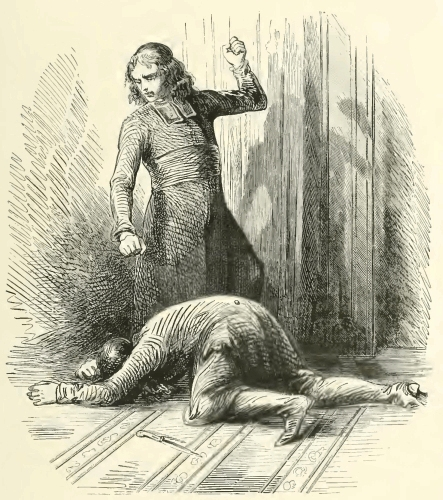
\includegraphics[width=\textwidth]{40162m.jpg}
\end{figure}

“Rise!” said he. Caderousse rose.

“What a wrist you have, reverend sir!” said Caderousse, stroking his
arm, all bruised by the fleshy pincers which had held it; “what a
wrist!”

“Silence! God gives me strength to overcome a wild beast like you; in
the name of that God I act,—remember that, wretch,—and to spare thee at
this moment is still serving him.”

“Oh!” said Caderousse, groaning with pain.

“Take this pen and paper, and write what I dictate.”

“I don’t know how to write, reverend sir.”

“You lie! Take this pen, and write!”

Caderousse, awed by the superior power of the abbé, sat down and wrote:

\begin{quote}
{\small“Sir,—The man whom you are receiving at your house, and to whom you
intend to marry your daughter, is a felon who escaped with me from
confinement at Toulon. He was No. 59, and I No. 58. He was called
Benedetto, but he is ignorant of his real name, having never known his
parents.”}
\end{quote}

“Sign it!” continued the count.

“But would you ruin me?”

“If I sought your ruin, fool, I should drag you to the first
guard-house; besides, when that note is delivered, in all probability
you will have no more to fear. Sign it, then!”

Caderousse signed it.

“The address, ‘To monsieur the Baron Danglars, banker, Rue de la
Chaussée d’Antin.’”

Caderousse wrote the address. The abbé took the note.

“Now,” said he, “that suffices—begone!”

“Which way?”

“The way you came.”

“You wish me to get out at that window?”

“You got in very well.”

“Oh, you have some design against me, reverend sir.”

“Idiot! what design can I have?”

“Why, then, not let me out by the door?”

“What would be the advantage of waking the porter?”

“Ah, reverend sir, tell me, do you wish me dead?”

“I wish what God wills.”

“But swear that you will not strike me as I go down.”

“Cowardly fool!”

“What do you intend doing with me?”

“I ask you what can I do? I have tried to make you a happy man, and you
have turned out a murderer.”

“Oh, monsieur,” said Caderousse, “make one more attempt—try me once
more!”

“I will,” said the count. “Listen—you know if I may be relied on.”

“Yes,” said Caderousse.

“If you arrive safely at home——”

“What have I to fear, except from you?”

“If you reach your home safely, leave Paris, leave France, and wherever
you may be, so long as you conduct yourself well, I will send you a
small annuity; for, if you return home safely, then——”

“Then?” asked Caderousse, shuddering.

\begin{figure}[ht]
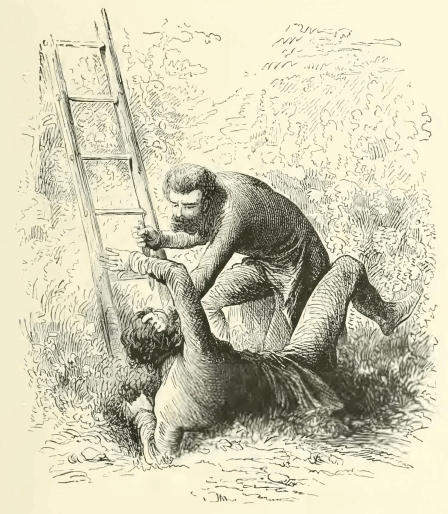
\includegraphics[width=\textwidth]{40164m.jpg}
\end{figure}

“Then I shall believe God has forgiven you, and I will forgive you
too.”

“As true as I am a Christian,” stammered Caderousse, “you will make me
die of fright!”

“Now begone,” said the count, pointing to the window.

Caderousse, scarcely yet relying on this promise, put his legs out of
the window and stood on the ladder.

“Now go down,” said the abbé, folding his arms. Understanding he had
nothing more to fear from him, Caderousse began to go down. Then the
count brought the taper to the window, that it might be seen in the
Champs-Élysées that a man was getting out of the window while another
held a light.

“What are you doing, reverend sir? Suppose a watchman should pass?” And
he blew out the light. He then descended, but it was only when he felt
his foot touch the ground that he was satisfied of his safety.

Monte Cristo returned to his bedroom, and, glancing rapidly from the
garden to the street, he saw first Caderousse, who after walking to the
end of the garden, fixed his ladder against the wall at a different
part from where he came in. The count then looking over into the
street, saw the man who appeared to be waiting run in the same
direction, and place himself against the angle of the wall where
Caderousse would come over. Caderousse climbed the ladder slowly, and
looked over the coping to see if the street was quiet. No one could be
seen or heard. The clock of the Invalides struck one. Then Caderousse
sat astride the coping, and drawing up his ladder passed it over the
wall; then he began to descend, or rather to slide down by the two
stanchions, which he did with an ease which proved how accustomed he
was to the exercise. But, once started, he could not stop. In vain did
he see a man start from the shadow when he was halfway down—in vain did
he see an arm raised as he touched the ground.

Before he could defend himself that arm struck him so violently in the
back that he let go the ladder, crying, “Help!” A second blow struck
him almost immediately in the side, and he fell, calling, “Help,
murder!” Then, as he rolled on the ground, his adversary seized him by
the hair, and struck him a third blow in the chest.

This time Caderousse endeavored to call again, but he could only utter
a groan, and he shuddered as the blood flowed from his three wounds.
The assassin, finding that he no longer cried out, lifted his head up
by the hair; his eyes were closed, and the mouth was distorted. The
murderer, supposing him dead, let fall his head and disappeared.

Then Caderousse, feeling that he was leaving him, raised himself on his
elbow, and with a dying voice cried with great effort:

“Murder! I am dying! Help, reverend sir,—help!”

This mournful appeal pierced the darkness. The door of the
back-staircase opened, then the side-gate of the garden, and Ali and
his master were on the spot with lights.
